\documentclass[11pt]{article}
\usepackage[spanish]{babel}
\usepackage[utf8]{inputenc}
\usepackage[T1]{fontenc}
\usepackage[margin=1in]{geometry}
\usepackage{graphicx}
\usepackage{float}
\usepackage{multirow}
\usepackage{array}
\usepackage{tabularx}
\usepackage{enumitem}

\setlist[itemize]{itemsep=0.35em, topsep=0.35em}

\title{Apunte de Electrónica Digital III}
\author{Nombre y apellido}
\date{\today}

\begin{document}

\maketitle
\tableofcontents

\section{Descripción}
\subsection{Introducción}
Este documento corresponde al apunte de la materia Electrónica Digital III y está centrado en el estudio del microprocesador LPC1769, basado en la arquitectura ARM Cortex-M3. Está pensado para aplicaciones embebidas y requiere un alto nivel de integración y bajo nivel de disipación de energía.

\subsection{Características}
\begin{itemize}
  \item CPU ARM Cortex-M3 de hasta 120 MHz con soporte de interrupciones (NVIC) y bajo consumo.
  \item Hasta 512 KB de flash y 64 KB de RAM, con aceleración para acceso rápido a código y datos.
  \item Periféricos de comunicación completos: Ethernet, USB 2.0 OTG, CAN, UART, SPI, SSP, I2C e I2S.
  \item Interfaces analógicas integradas: ADC de 12 bits, DAC de 10 bits y sensores/monitores internos.
  \item Temporización y control: timers de 32 bits, PWM, RTC de bajo consumo y watchdog.
  \item Entradas/salidas versátiles: GPIO de alta velocidad, captura/comparación y codificador en cuadratura.
  \item Enfoque en eficiencia energética con modos Sleep, Deep-sleep, Power-down y Deep power-down.
  \item Soporte de depuración y trazado: JTAG/SWD, ETM y emulación en tiempo real.
  \item Reloj flexible: oscilador interno/externo, PLL y \textit{clock output} para supervisión del sistema.
  \item Encapsulados LQFP y BGA compactos, orientados a aplicaciones embebidas industriales.
\end{itemize}

\setcounter{subsection}{4}
\subsection{Diagrama de bloques}
\begin{figure}[H]
  \centering
  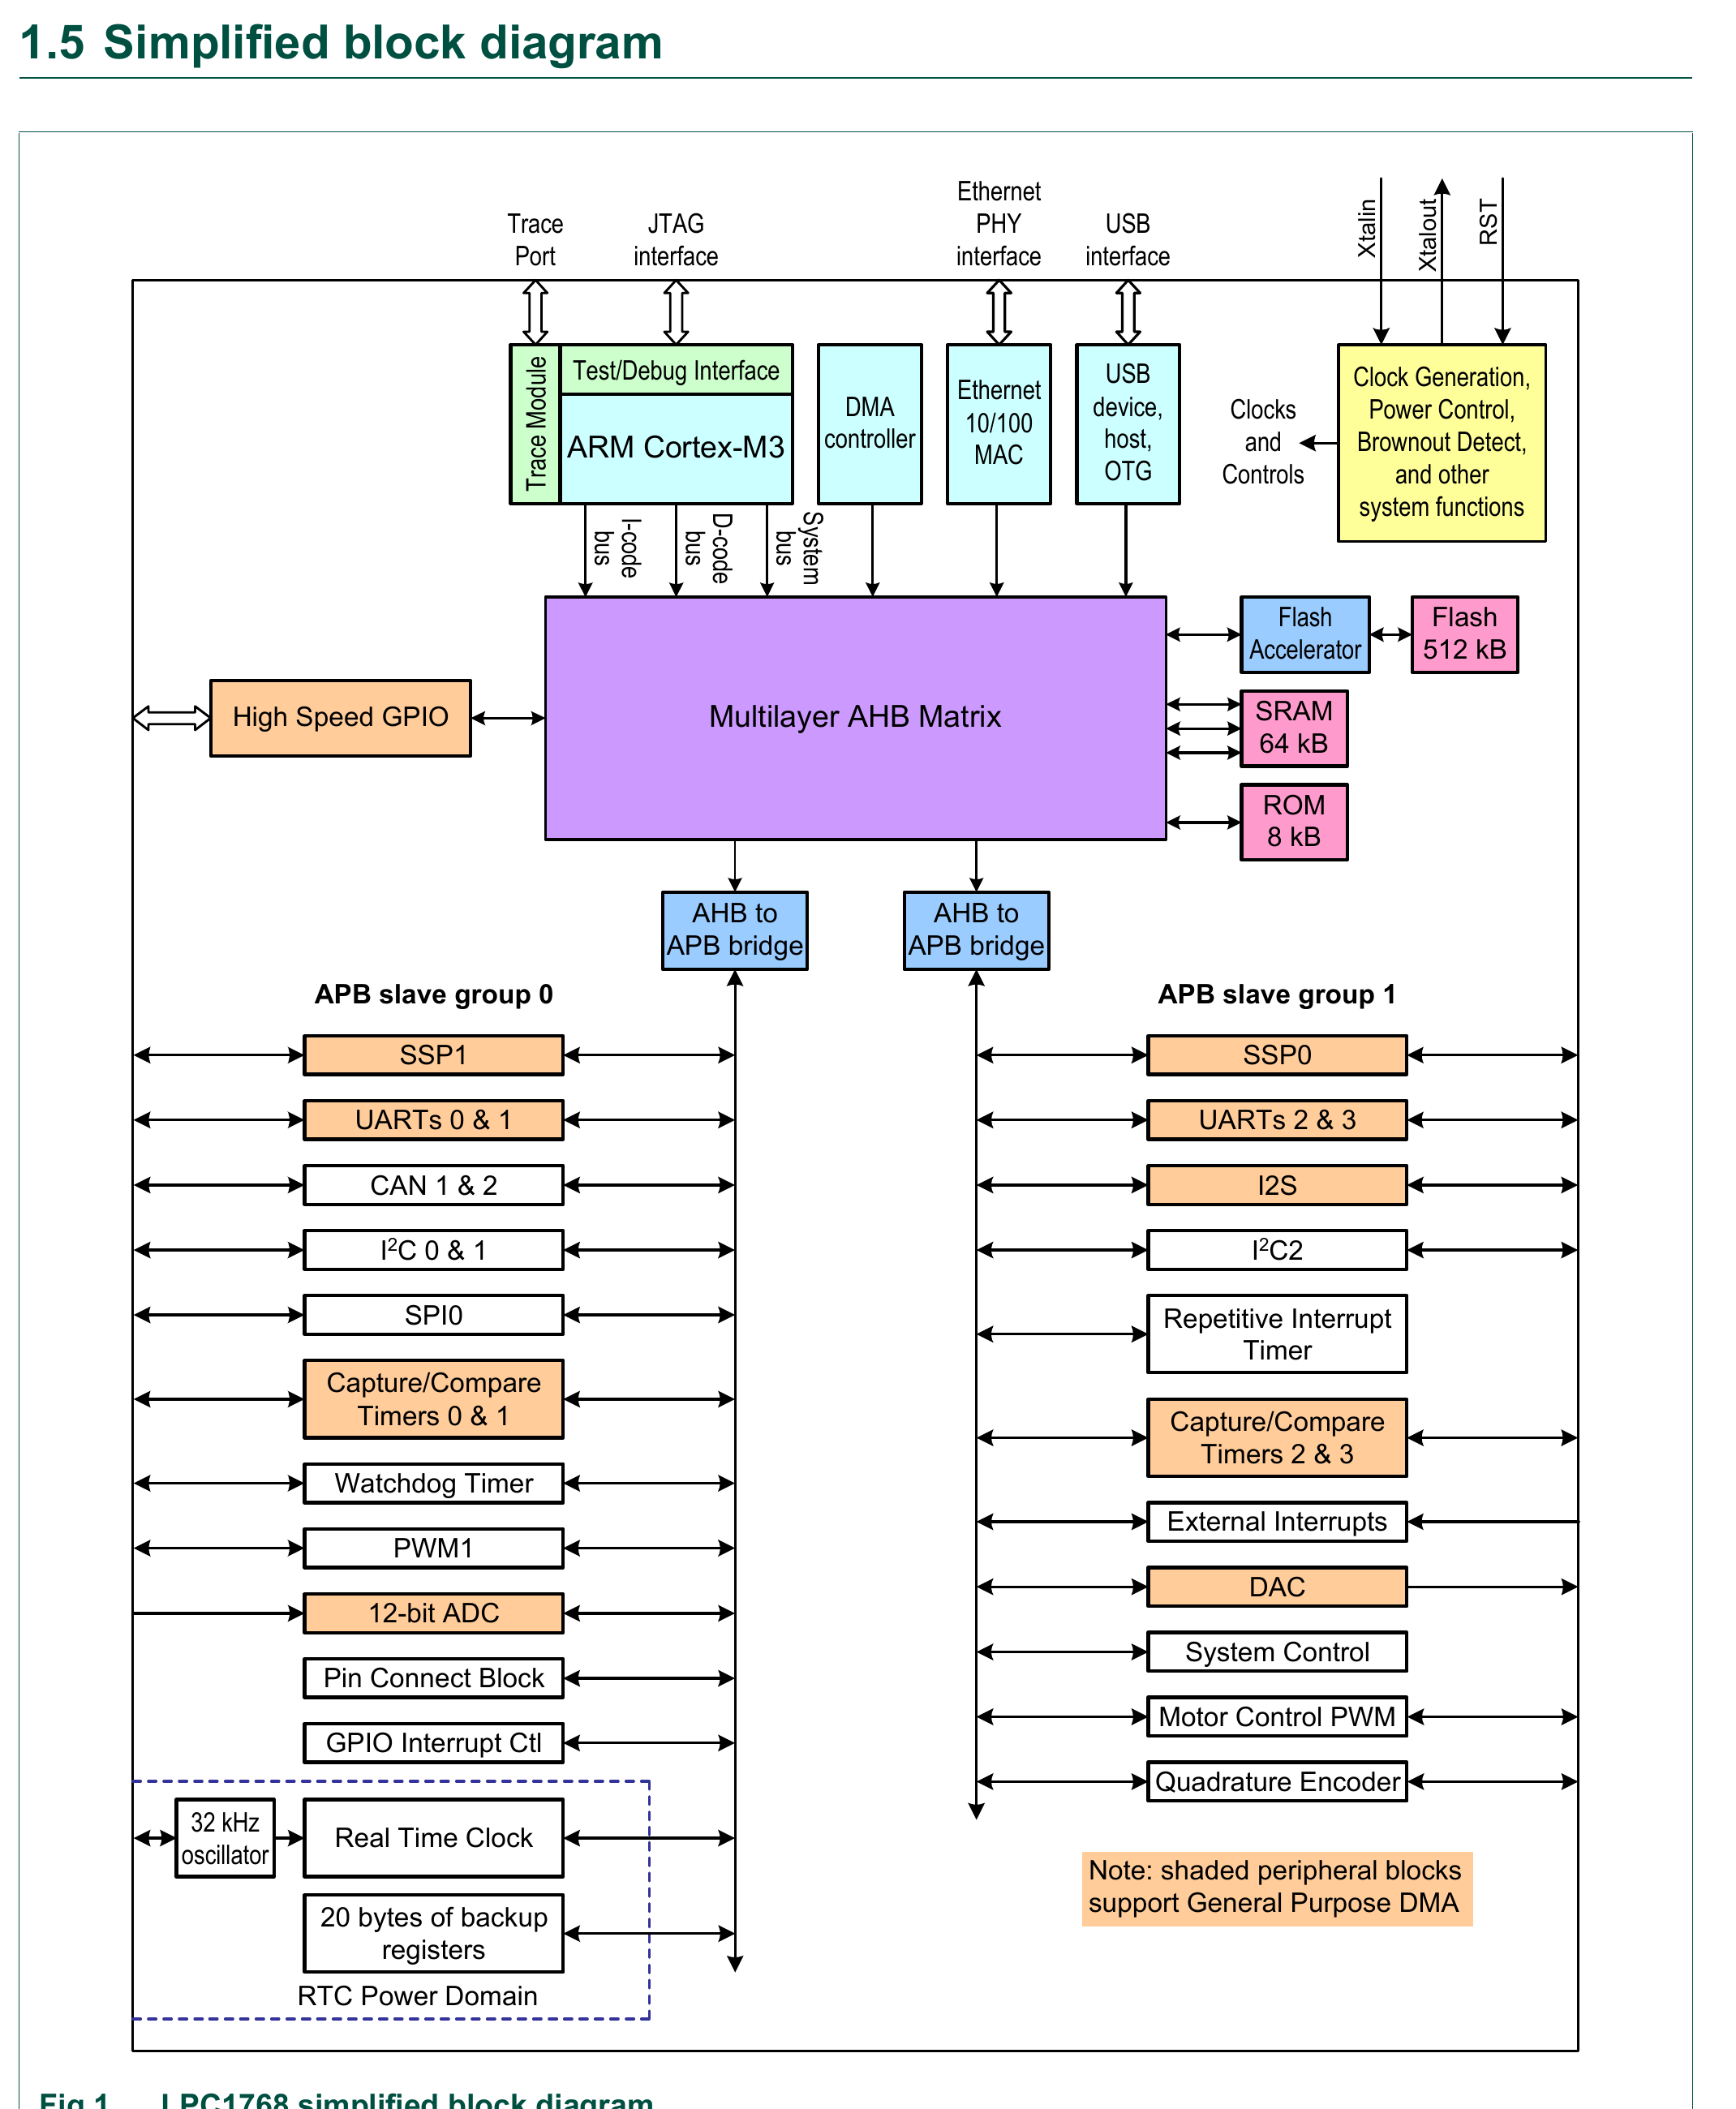
\includegraphics[width=0.93\textwidth]{images/lpc1769_block_diagram.png}
  \caption{Diagrama de bloques simplificado del LPC1769.}
\end{figure}

\subsection{Vista general de arquitectura}
\begin{figure}[H]
  \centering
  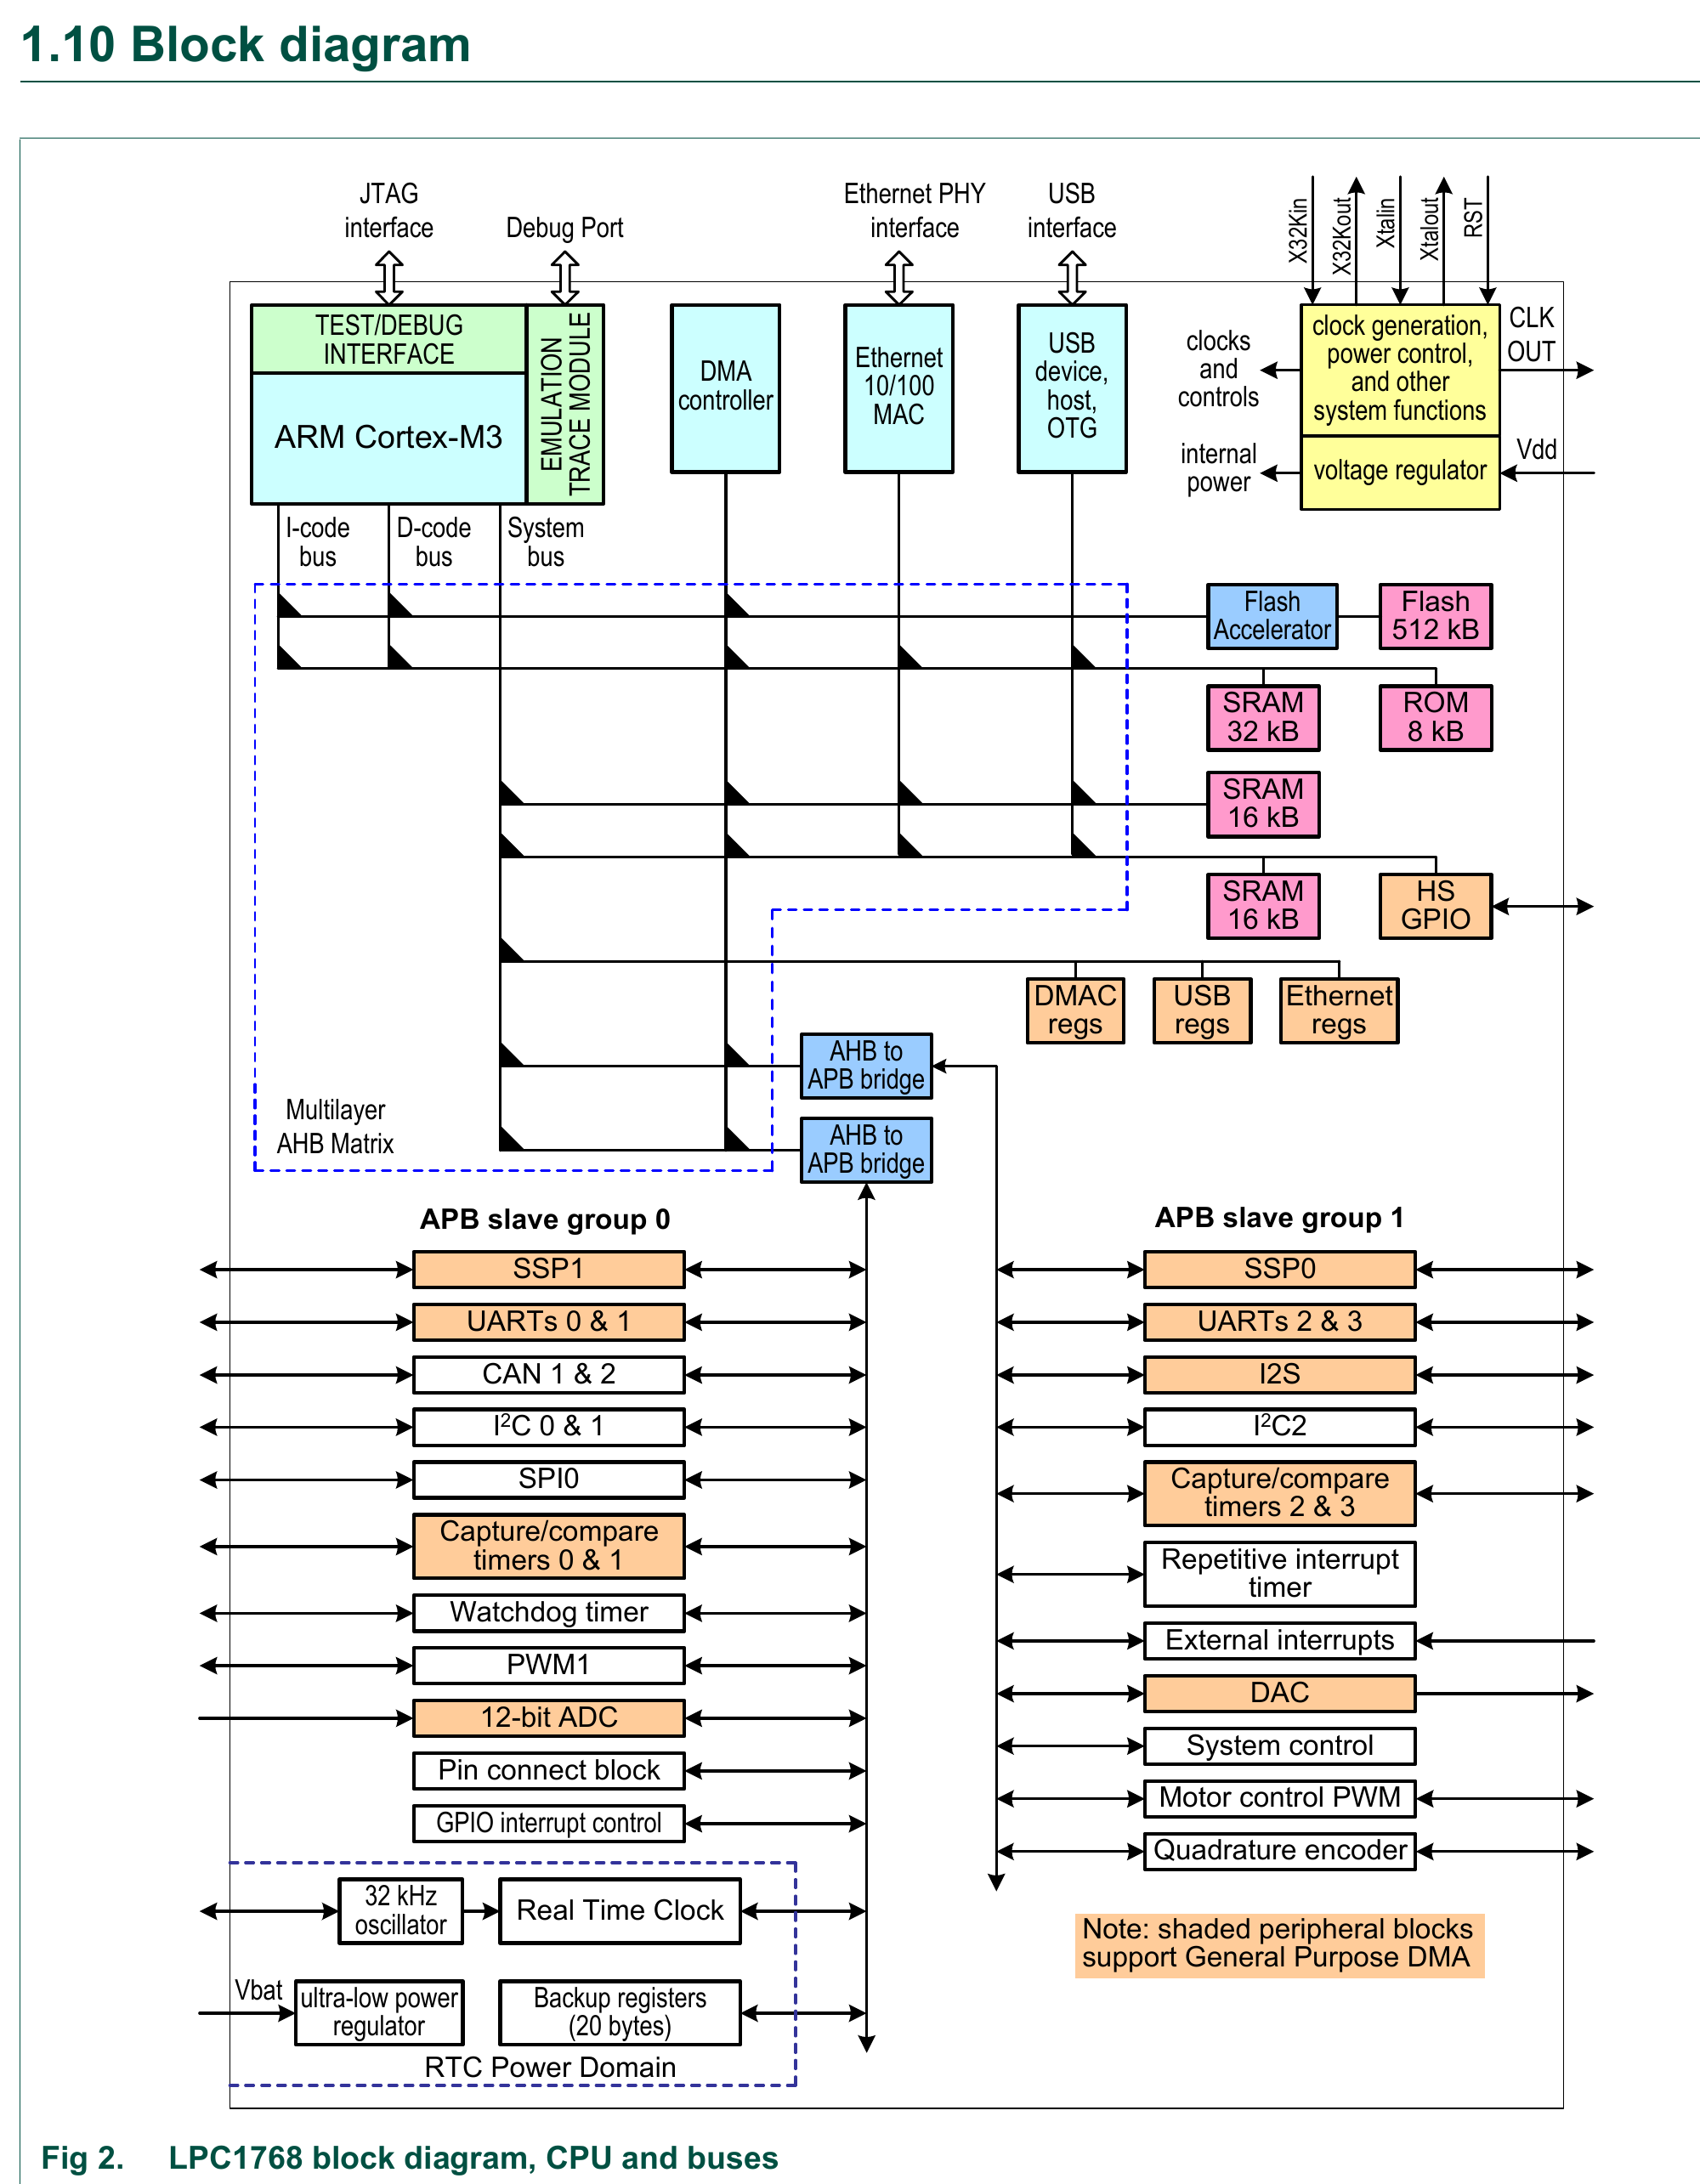
\includegraphics[width=0.83\textwidth]{images/lpc1769_ahb_matrix_detailed.png}
  \caption{Diagrama de bloques detallado con matriz AHB multicapa.}
\end{figure}

\begin{itemize}
  \item \textbf{Buses del núcleo ARM Cortex-M3:} El procesador usa tres buses AHB-Lite (\textit{Advanced High-performance Bus}): un bus de sistema y dos buses rápidos, \textbf{I-code} (instrucciones) y \textbf{D-code} (datos). Esta separación permite ejecutar accesos simultáneos cuando apuntan a periféricos distintos.

  \item \textbf{Matriz AHB multicapa:} El LPC17xx integra una matriz AHB multicapa que conecta los maestros de bus (CPU, DMA, Ethernet, USB, etc.) con distintos puertos esclavos. Así, varios accesos pueden ocurrir en paralelo y se mejora el rendimiento global.

  \item \textbf{Conexión de periféricos APB:} Los periféricos APB (\textit{Advanced Peripheral Bus}) se enlazan mediante dos buses APB conectados a puertos esclavos separados de la matriz AHB. Esto reduce colisiones entre CPU y DMA (Acceso Directo a Memoria).

  \item \textbf{Búfer de escritura APB:} Los puentes APB almacenan escrituras en búfer, permitiendo que la CPU o el DMA continúen su ejecución sin esperar a que cada escritura finalice.
\end{itemize}

\subsection{Opciones de configuración del Cortex-M3}
\begin{itemize}
  \item \textbf{Técnicas de segmentación (pipeline):} El núcleo aplica pipeline para mantener activos los bloques de procesamiento y memoria. En condiciones normales, mientras una instrucción se ejecuta, la siguiente se decodifica y una tercera se busca en memoria.

  \item \textbf{Versión del núcleo:} Los LPC17xx usan la versión \textbf{r2p0} del Cortex-M3, que integra opciones de sistema configurables:
  \begin{itemize}
    \item \textbf{NVIC (Nested Vectored Interrupt Controller):} controlador de interrupciones con temporizador SysTick.
    \item \textbf{WIC (Wakeup Interrupt Controller):} habilita un despertar más eficiente desde modos de bajo consumo.
    \item \textbf{MPU (Memory Protection Unit):} unidad de protección de memoria incorporada.
    \item \textbf{ROM Table:} expone a herramientas externas las direcciones de componentes de depuración.
  \end{itemize}

  \item \textbf{Opciones de depuración (Debug):} La CPU incorpora funciones configurables para diagnóstico y depuración de fallas, también asociadas al conjunto de opciones r2p0.
\end{itemize}

\subsection{Sistema de memoria flash en chip}
\begin{itemize}
  \item \textbf{Capacidad:} El LPC17xx integra hasta \textbf{512 kB de memoria flash} en el propio chip.
  \item \textbf{Rendimiento:} Incluye un \textbf{acelerador de flash} que mejora el acceso cuando trabaja junto con los buses rápidos AHB-Lite.
  \item \textbf{Uso:} La flash puede utilizarse tanto para \textbf{código} como para \textbf{datos}, aportando flexibilidad en aplicaciones embebidas.
  \item \textbf{Programación y actualización:} Puede programarse \textit{in-system} por puerto serie, y la propia aplicación puede \textbf{borrar/programar flash en ejecución}, facilitando actualizaciones de firmware en campo y almacenamiento de datos.
\end{itemize}

\subsection{Memoria SRAM en chip}
\begin{itemize}
  \item \textbf{32 kB de SRAM local:} conectada directamente a los buses locales de la CPU (I-code/D-code), lo que permite acceso de alta velocidad.
  \item \textbf{32 kB de SRAM AHB:} organizada en dos bloques de 16 kB y conectada al bus periférico AHB.
\end{itemize}

\section{Mapeo de memoria del LPC1769}
\subsection{Mapa de memoria y direccionamiento de periféricos}
\begin{table}[H]
  \centering
  \small
  \renewcommand{\arraystretch}{1.2}
  \setlength{\tabcolsep}{6pt}
  \caption{Uso de memoria y regiones del LPC1769}
  \begin{tabularx}{\textwidth}{|>{\raggedright\arraybackslash}p{0.22\textwidth}|>{\raggedright\arraybackslash}p{0.23\textwidth}|>{\raggedright\arraybackslash}X|}
    \hline
    \textbf{Rango de direcciones} & \textbf{Uso general} & \textbf{Detalle de región y descripción} \\
    \hline
    \multirow{3}{=}{\texttt{0x0000\,0000} a \\ \texttt{0x1FFF\,FFFF}}
      & Memoria no volátil en chip & 0x0000\,0000 -- 0x0007\,FFFF: para LPC1769 con 512 kB de memoria flash. \\
    \cline{2-3}
      & SRAM en chip & 0x1000\,0000 -- 0x1000\,7FFF: 32 kB de SRAM local. \\
    \cline{2-3}
      & Boot ROM & 0x1FFF\,0000 -- 0x1FFF\,1FFF: 8 kB de Boot ROM con servicios de flash. \\
    \hline
    \multirow{3}{=}{\texttt{0x2000\,0000} a \\ \texttt{0x3FFF\,FFFF}}
      & SRAM en chip (uso típico de datos periféricos) & 0x2007\,C000 -- 0x2007\,FFFF: banco AHB SRAM 0 (16 kB), presente en dispositivos con 32 kB o 64 kB de SRAM total. \\
    \cline{2-3}
      & SRAM en chip (uso típico de datos periféricos) & 0x2008\,0000 -- 0x2008\,3FFF: banco AHB SRAM 1 (16 kB), presente en dispositivos con 64 kB de SRAM total. \\
    \cline{2-3}
      & GPIO & 0x2009\,C000 -- 0x2009\,FFFF: registros GPIO. \\
    \hline
    \multirow{3}{=}{\texttt{0x4000\,0000} a \\ \texttt{0x5FFF\,FFFF}}
      & Periféricos APB & 0x4000\,0000 -- 0x4007\,FFFF: periféricos APB0, hasta 32 bloques de 16 kB cada uno. \\
    \cline{2-3}
      & Periféricos APB & 0x4008\,0000 -- 0x400F\,FFFF: periféricos APB1, hasta 32 bloques de 16 kB cada uno. \\
    \cline{2-3}
      & Periféricos AHB & 0x5000\,0000 -- 0x501F\,FFFF: controlador DMA, interfaz Ethernet e interfaz USB. \\
    \hline
    \texttt{0xE000\,0000} a \\ \texttt{0xE00F\,FFFF}
      & Bus de periféricos privados del Cortex-M3 & 0xE000\,0000 -- 0xE00F\,FFFF: funciones del Cortex-M3, incluido NVIC y temporizador SysTick. \\
    \hline
  \end{tabularx}
\end{table}

\subsection{Mapa de memoria}
\begin{figure}[H]
  \centering
  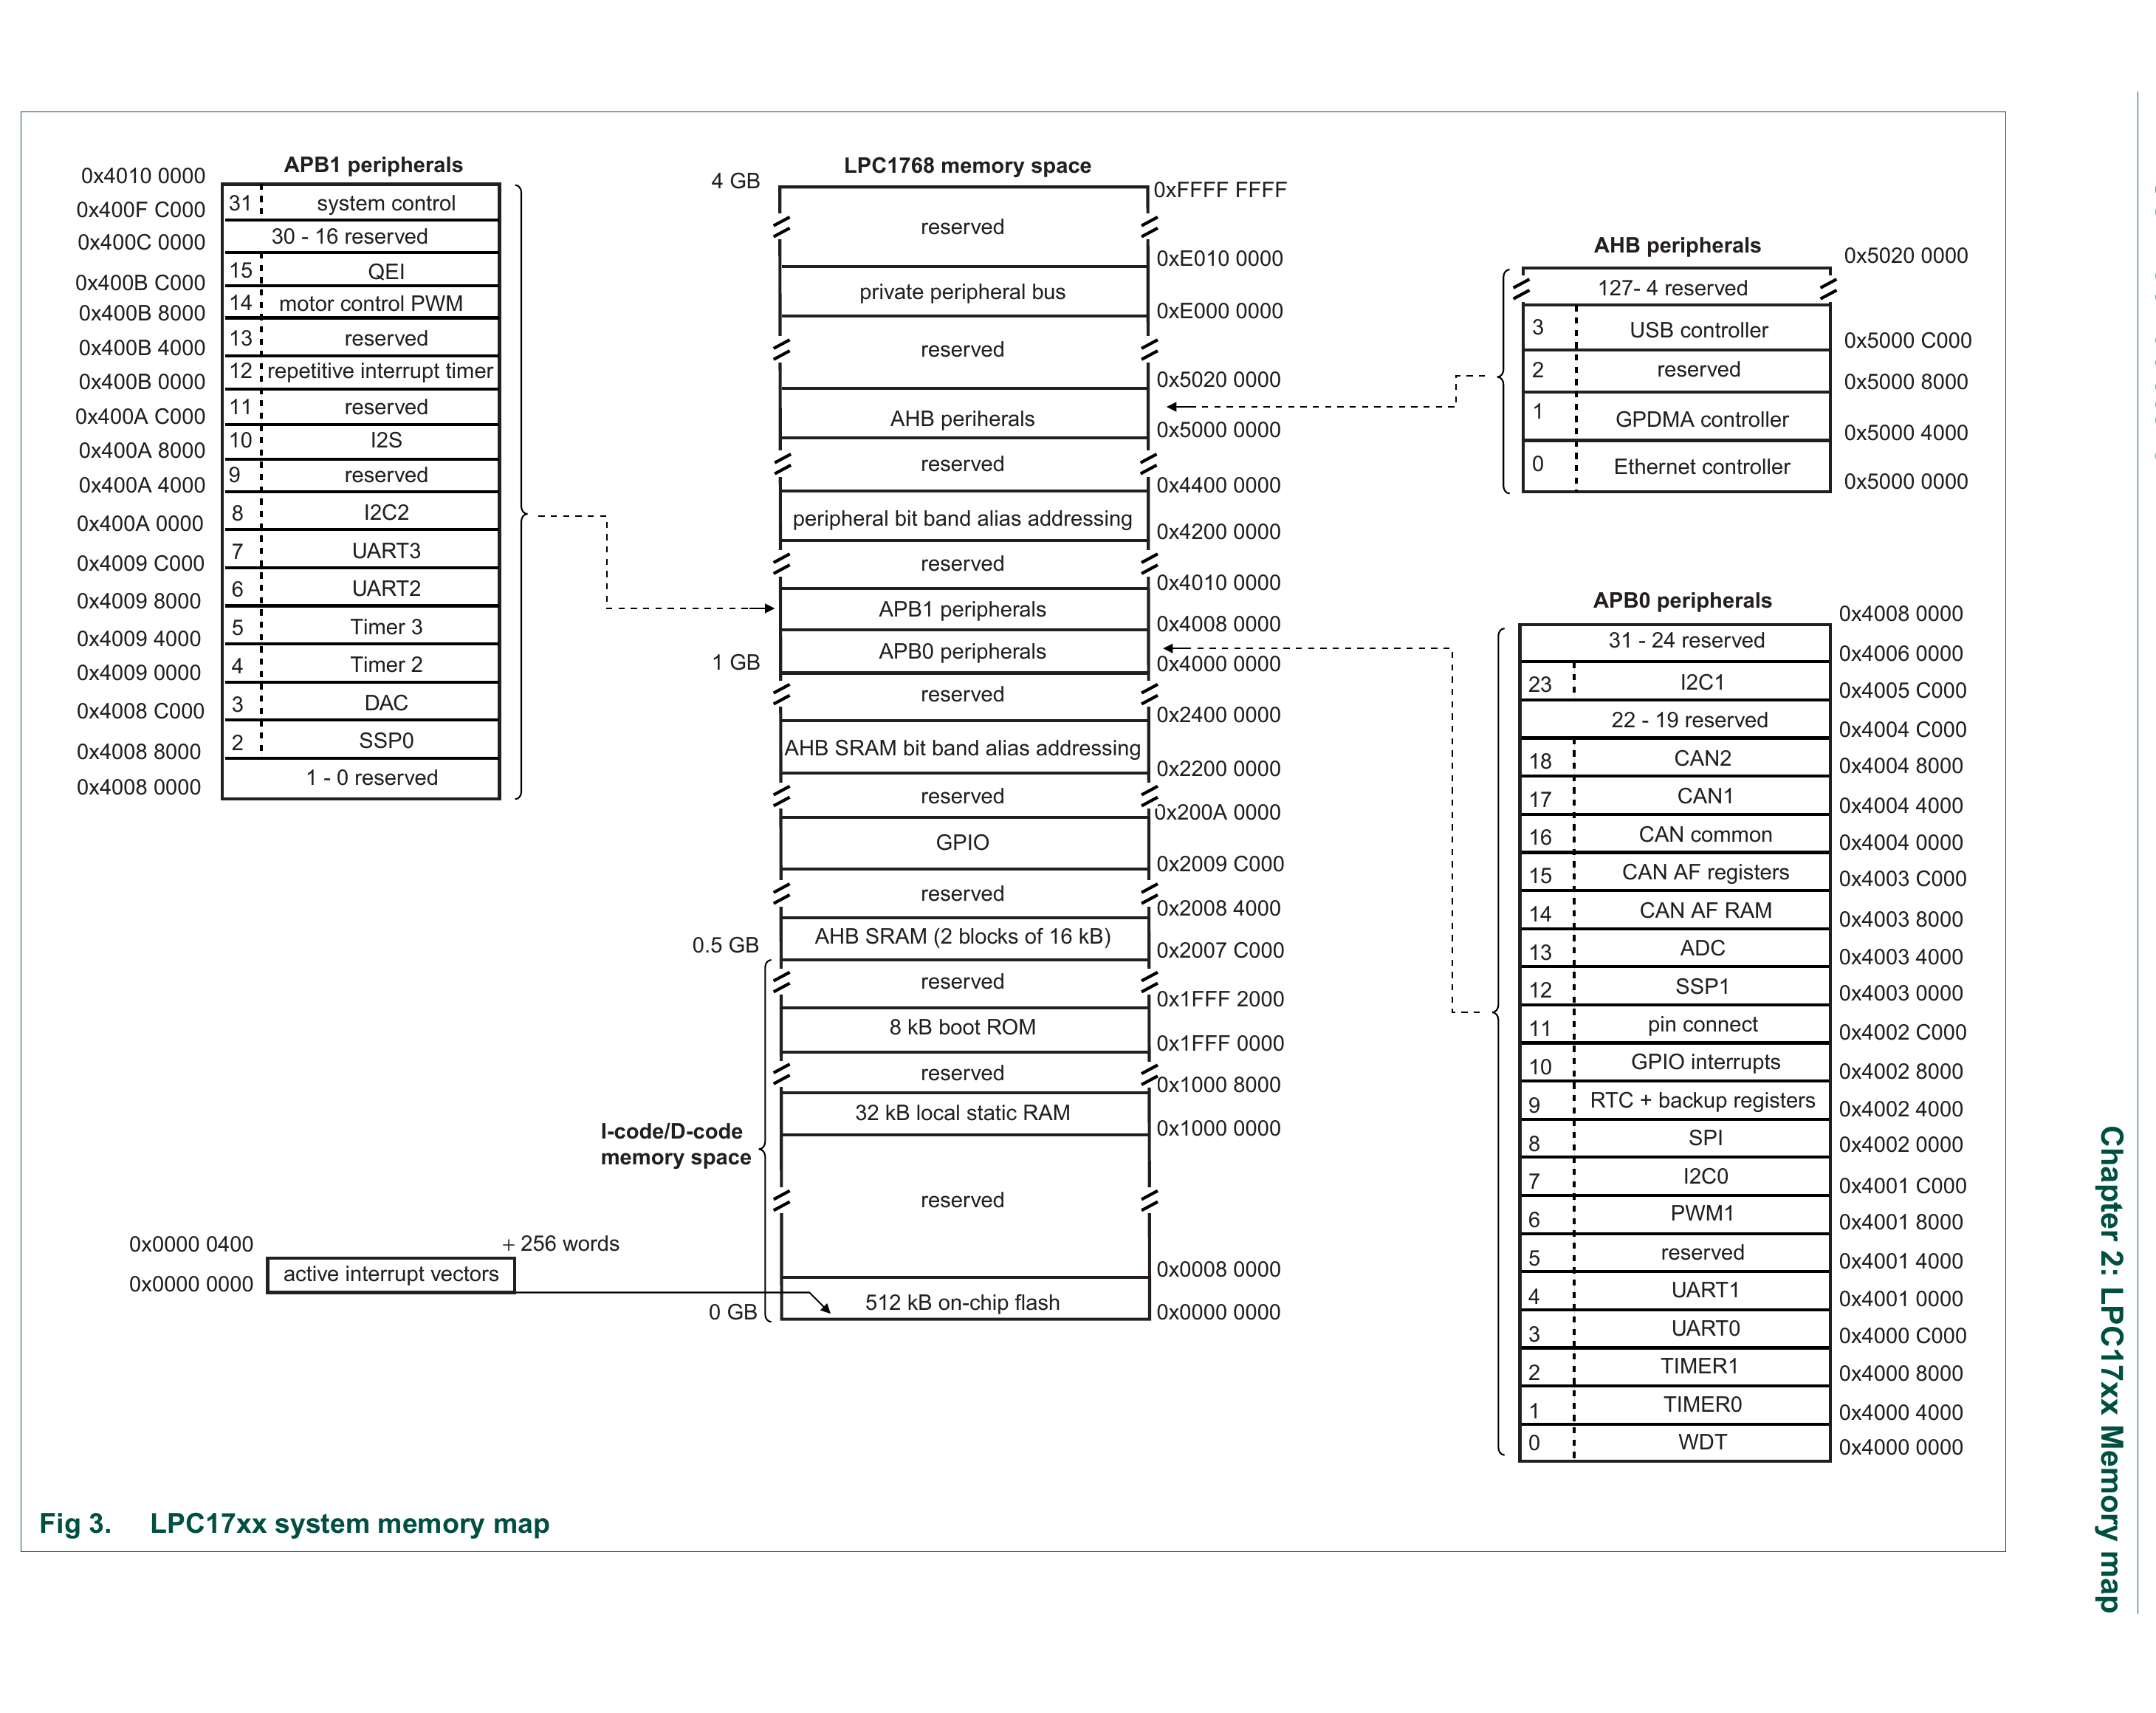
\includegraphics[width=0.98\textwidth]{images/lpc17xx_system_memory_map.png}
  \caption{Mapa de memoria del sistema LPC17xx.}
\end{figure}

\subsection{Direcciones de periféricos APB}
En esta sección se resume el mapeo de direcciones base de los periféricos conectados a los buses \textbf{APB0} y \textbf{APB1}. Cada bloque APB ocupa un espacio de \textbf{16 kB} y, en general, los registros de cada periférico no utilizan todo ese rango. Por este motivo, en varios casos aparecen direcciones \textit{aliasadas} o repetidas dentro del mismo bloque de 16 kB.

\begin{table}[H]
  \centering
  \small
  \renewcommand{\arraystretch}{1.1}
  \setlength{\tabcolsep}{4pt}
  \caption{Periféricos APB0 y direcciones base}
  \begin{tabularx}{0.94\textwidth}{|>{\raggedright\arraybackslash}p{0.14\textwidth}|>{\raggedright\arraybackslash}p{0.20\textwidth}|>{\raggedright\arraybackslash}X|}
    \hline
    \textbf{Periférico APB0} & \textbf{Dirección base} & \textbf{Nombre del periférico} \\
    \hline
    0 & \texttt{0x4000\,0000} & Watchdog timer (WDT) \\
    1 & \texttt{0x4000\,4000} & Timer 0 \\
    2 & \texttt{0x4000\,8000} & Timer 1 \\
    3 & \texttt{0x4000\,C000} & UART0 \\
    4 & \texttt{0x4001\,0000} & UART1 \\
    5 & \texttt{0x4001\,4000} & Reservado \\
    6 & \texttt{0x4001\,8000} & PWM1 \\
    7 & \texttt{0x4001\,C000} & I$^2$C0 \\
    8 & \texttt{0x4002\,0000} & SPI \\
    9 & \texttt{0x4002\,4000} & RTC \\
    10 & \texttt{0x4002\,8000} & Interrupciones GPIO \\
    11 & \texttt{0x4002\,C000} & Pin connect block \\
    12 & \texttt{0x4003\,0000} & SSP1 \\
    13 & \texttt{0x4003\,4000} & ADC \\
    14 & \texttt{0x4003\,8000} & CAN Acceptance Filter RAM \\
    15 & \texttt{0x4003\,C000} & CAN Acceptance Filter Registers \\
    16 & \texttt{0x4004\,0000} & CAN Common Registers \\
    17 & \texttt{0x4004\,4000} & CAN Controller 1 \\
    18 & \texttt{0x4004\,8000} & CAN Controller 2 \\
    19 a 22 & \texttt{0x4004\,C000} a \texttt{0x4005\,8000} & Reservado \\
    23 & \texttt{0x4005\,C000} & I$^2$C1 \\
    24 a 31 & \texttt{0x4006\,0000} a \texttt{0x4007\,C000} & Reservado \\
    \hline
  \end{tabularx}
\end{table}

\begin{table}[H]
  \centering
  \small
  \renewcommand{\arraystretch}{1.1}
  \setlength{\tabcolsep}{4pt}
  \caption{Periféricos APB1 y direcciones base}
  \begin{tabularx}{0.94\textwidth}{|>{\raggedright\arraybackslash}p{0.14\textwidth}|>{\raggedright\arraybackslash}p{0.20\textwidth}|>{\raggedright\arraybackslash}X|}
    \hline
    \textbf{Periférico APB1} & \textbf{Dirección base} & \textbf{Nombre del periférico} \\
    \hline
    0 & \texttt{0x4008\,0000} & Reservado \\
    1 & \texttt{0x4008\,4000} & Reservado \\
    2 & \texttt{0x4008\,8000} & SSP0 \\
    3 & \texttt{0x4008\,C000} & DAC \\
    4 & \texttt{0x4009\,0000} & Timer 2 \\
    5 & \texttt{0x4009\,4000} & Timer 3 \\
    6 & \texttt{0x4009\,8000} & UART2 \\
    7 & \texttt{0x4009\,C000} & UART3 \\
    8 & \texttt{0x400A\,0000} & I$^2$C2 \\
    9 & \texttt{0x400A\,4000} & Reservado \\
    10 & \texttt{0x400A\,8000} & I$^2$S \\
    11 & \texttt{0x400A\,C000} & Reservado \\
    12 & \texttt{0x400B\,0000} & Repetitive interrupt timer \\
    13 & \texttt{0x400B\,4000} & Reservado \\
    14 & \texttt{0x400B\,8000} & Motor control PWM \\
    15 & \texttt{0x400B\,C000} & Quadrature Encoder Interface \\
    16 a 30 & \texttt{0x400C\,0000} a \texttt{0x400F\,8000} & Reservado \\
    31 & \texttt{0x400F\,C000} & System control \\
    \hline
  \end{tabularx}
\end{table}

\subsection{Remapeo de memoria}
El Cortex-M3 permite \textbf{remapear la tabla de vectores de interrupción} a distintas ubicaciones del mapa de memoria mediante el \textit{Vector Table Offset Register} (VTOR). Esto facilita ubicar la tabla en la región más conveniente para la aplicación (por ejemplo, en flash o SRAM).

Además, tras un \textbf{reinicio por hardware}, la \textbf{Boot ROM} se mapea temporalmente en la dirección \texttt{0x0000\,0000}. En condiciones normales este comportamiento es transparente para el usuario; sin embargo, si un depurador detiene la ejecución inmediatamente después del reset, debe corregir ese mapeo para continuar con la depuración esperada.

\subsection{Arbitraje AHB}
La matriz AHB multicapa resuelve los accesos concurrentes de los distintos maestros del sistema mediante prioridades predefinidas. Por defecto, la \textbf{máxima prioridad} corresponde al bus de datos \textbf{D-code} del Cortex-M3, la \textbf{segunda prioridad} al bus de instrucciones \textbf{I-code}, y la \textbf{prioridad más baja} se comparte entre el resto de los maestros del sistema.

\subsection{Excepciones de fallo de bus}
El LPC17xx genera una \textbf{excepción de fallo de bus} cuando un programa intenta acceder a una dirección ubicada en una región de memoria \textbf{reservada o no asignada}. Estas regiones corresponden a zonas del mapa de memoria que no están implementadas en un modelo específico del chip.

\setcounter{section}{6}
\section{Configuración de pines LPC17xx}
\subsection{Configuración de pines LPC17xx}
\begin{figure}[H]
  \centering
  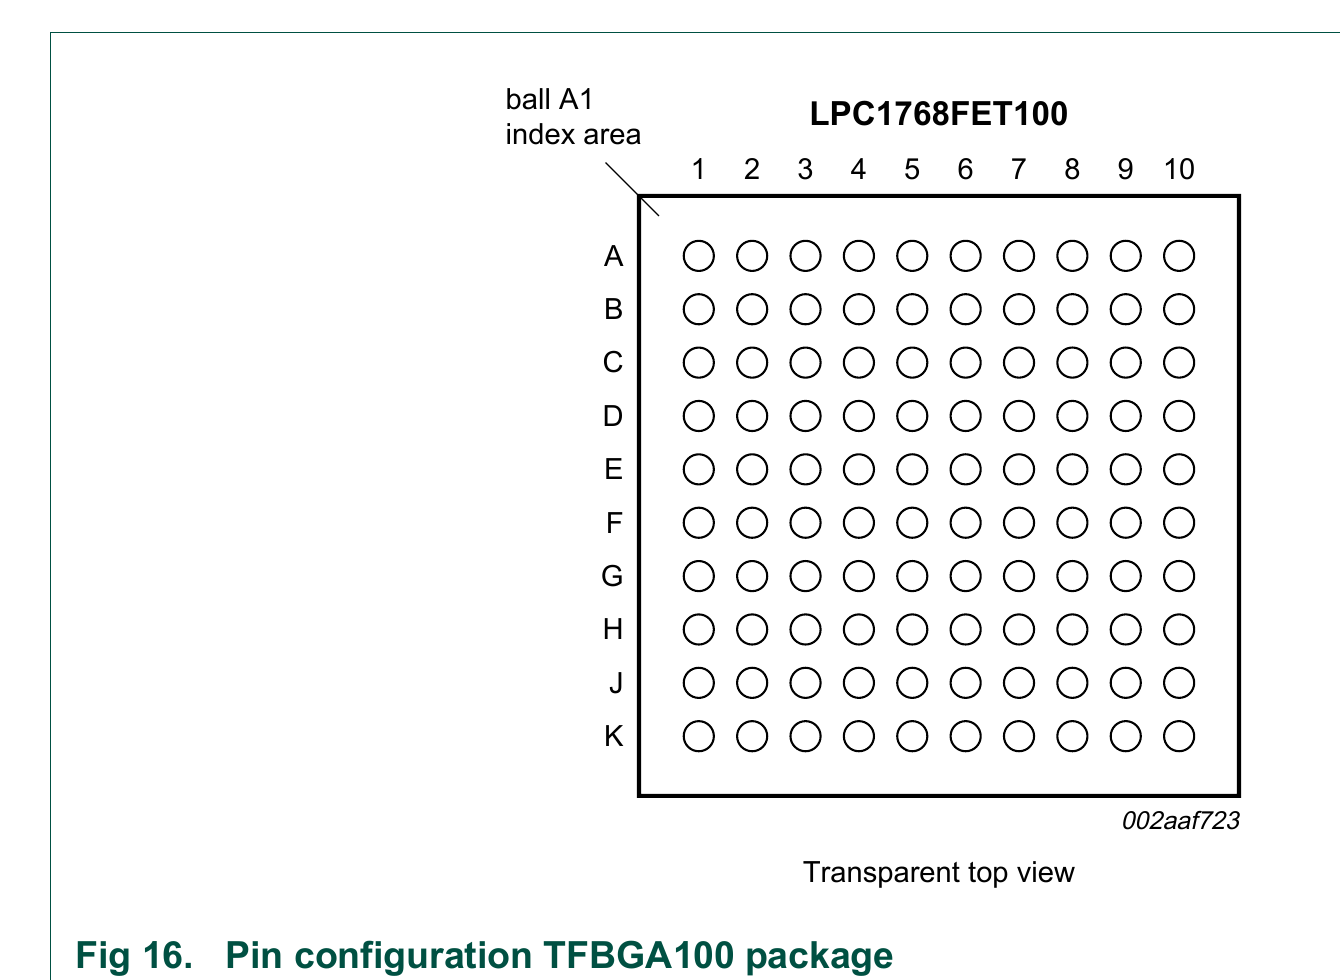
\includegraphics[width=0.93\textwidth]{images/lpc17xx_pin_configuration_tfbga100.png}
  \caption{Configuración de pines TFBGA100 del LPC176x.}
\end{figure}

\end{document}
